\documentclass[fleqn,10pt]{olplainarticle}
% Use option lineno for line numbers 
\title{What is the cause and effect in ship data analysis, when all I see is correlations?}

\author[1,2]{Martin Alexandersson}
\affil[1]{SSPA Sweden AB, Chalmers tvärgata 10, 41296 Gothenburg Sweden}
\affil[2]{Dept. of Mechanics and Maritime Sciences, Division of Marine Technology,
                                Chalmers University of Technology, Hörsalsvägen 7A, Gothenburg Sweden}

\keywords{Ship dynamics, Causal inference, Machine Learning}

%\begin{abstract}
%\end{abstract}

\begin{document}

\flushbottom
\maketitle
\thispagestyle{empty}

\section{Abstract}
% Move 1 - Background/introduction/situation
Statistical analysis or machine learning (ML) on real data can be used to propose changes in optimizing a system's behaviour. Before such changes could be proposed, determining the cause and effect relation between the variables -- causality -- is necessary.
The aim of standard statistical analysis or ML is to find trends or associations between variables. 
For these trends to be usable in optimization, we need to move one step further, also trying to find the causality.

% Move 2 - Present research/purpose
In this paper, causal inference is investigated on a dataset collected onboard the double ended ferry Uraniborg.
A previously observed trend with high correlation between thruster utilization (TU) and fuel consumption (FC) is investigated to see if there is direct causality, which can then be used to optimize the FC.

% Move 3 - Methods/materials/subjects/procedures
The inference was conducted with a controlled experiment onboard the ship, where the operation of the ship was altered between the captain and mate, every other journey.
% Move 4 - Results/findings
The experiment showed that there is most likely a direct causal relationship between the TU and FC.
An optimized TU, where only the aft thruster is utilized, is estimated to have between 9 and 17\% lower FC compared to the previous operation of the ship.

% Move 5 - Discussion/conclusion/significance
The experiment showed that it is possible to conduct a reasonably controlled experiment onboard a real ship during operation to infer the causality between the TU and FC.
This technique can be used within ship operational data analysis, where an associative analysis obtained with ML -- as correlations or regressions --  can be accompanied with a causal analysis, so that the identified association can be used to optimize the ship's operation.








\begin{figure}[!htb]
    \centering
    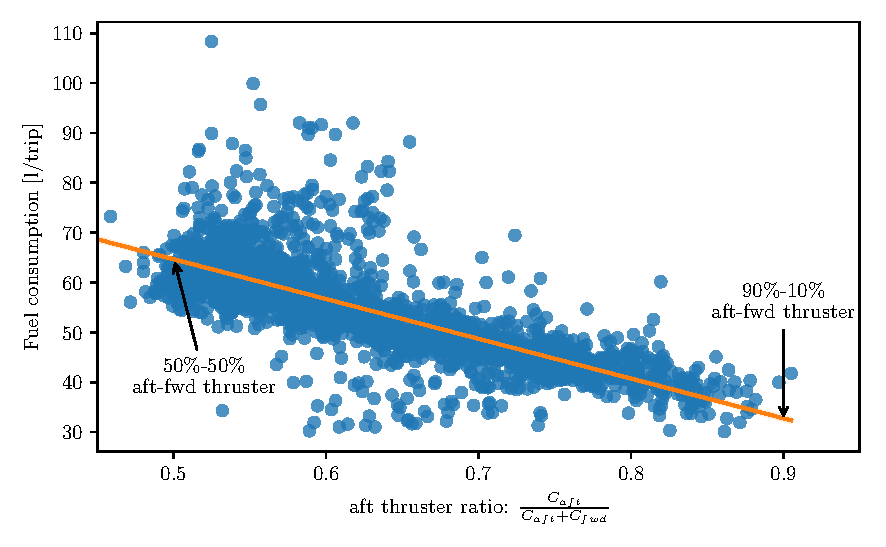
\includegraphics[width=\linewidth]{figures/correlation.pdf}
    \caption{Caption}
    \label{fig:my_label}
\end{figure}


A real example fcomes from the analysis of real operational data from a double ended ferry. Correlation between the thruster allocation, the utilization ratio between forward and aft thruster, was observed. Was this a direct causation or just a common causation, through a hidden variable like for instance the ocean current? 

In order to determine the causation an blinded experiment was carried out.


\bibliography{sample}

\end{document}